\section{Homework 3}

\noindent
Show all work.

\ben
\i Give examples of 
(a) a transverse wave 
and 
(b) a longitudinal wave.

\i Give examples of 
(a) a wave that requires a medium in which to travel and 
(b) a wave that travels in empty space.

\i Give an example that shows that waves transport energy.

\i A guitar string is stretched with a tension $\tau=50~{\rm lb}$.
It has a length $L=60~{\rm cm}$ and a mass $m=2~{\rm g}$.
Calculate the wave velocity for waves on the string, $v=\sqrt{\tau/\mu}$
where $\mu=m/L$.
(Note: Don't forget to convert lb to N, g to kg, and cm to m.)

\i Microwaves are examples of electromagnetic waves
which travel at 
$v=3\times 10^8~{\rm m/s}$ in vacuum.
If the frequency of the waves in a microwave oven
is $f=2.45\times 10^9~{\rm Hz}$, what is the corresponding
wavelength $\lambda$?
Is it short enough to fit inside the microwave
oven?
It should be.

\i Calculate the velocity of sound in air at a temperature of
(a)  $0~{}^\circ {\rm C}$,
(b) $20~{}^\circ {\rm C}$,
(c) $25~{}^\circ {\rm C}$, and
(d) $30~{}^\circ {\rm C}$.

\i Calculate the wavelength of sound in air at room temperature
for frequencies
(a) $f=20~{\rm Hz}$ and 
(b) $f=20~{\rm kHz}$.
(Recall: $v_{\rm air} = 346~{\rm m/s}$ at room temperature.)

\i Two notes with frequencies $f_1=440~{\rm Hz}$
and $f_2=441~{\rm Hz}$ are played simultaneously.
(a) What is the frequency of the sound that you hear?
(b) What is the beat frequency?

\i The standing wave pattern for the fundamental
frequency for a string fixed at both ends is
shown below.
Sketch the 2nd, 3rd, and 4th harmonics on the
following graphs.
If $L=1~{\rm m}$, what are the wavelengths of the
the fundamental frequency and these harmonics?
%
\begin{figure}[!h]
  \begin{center}
  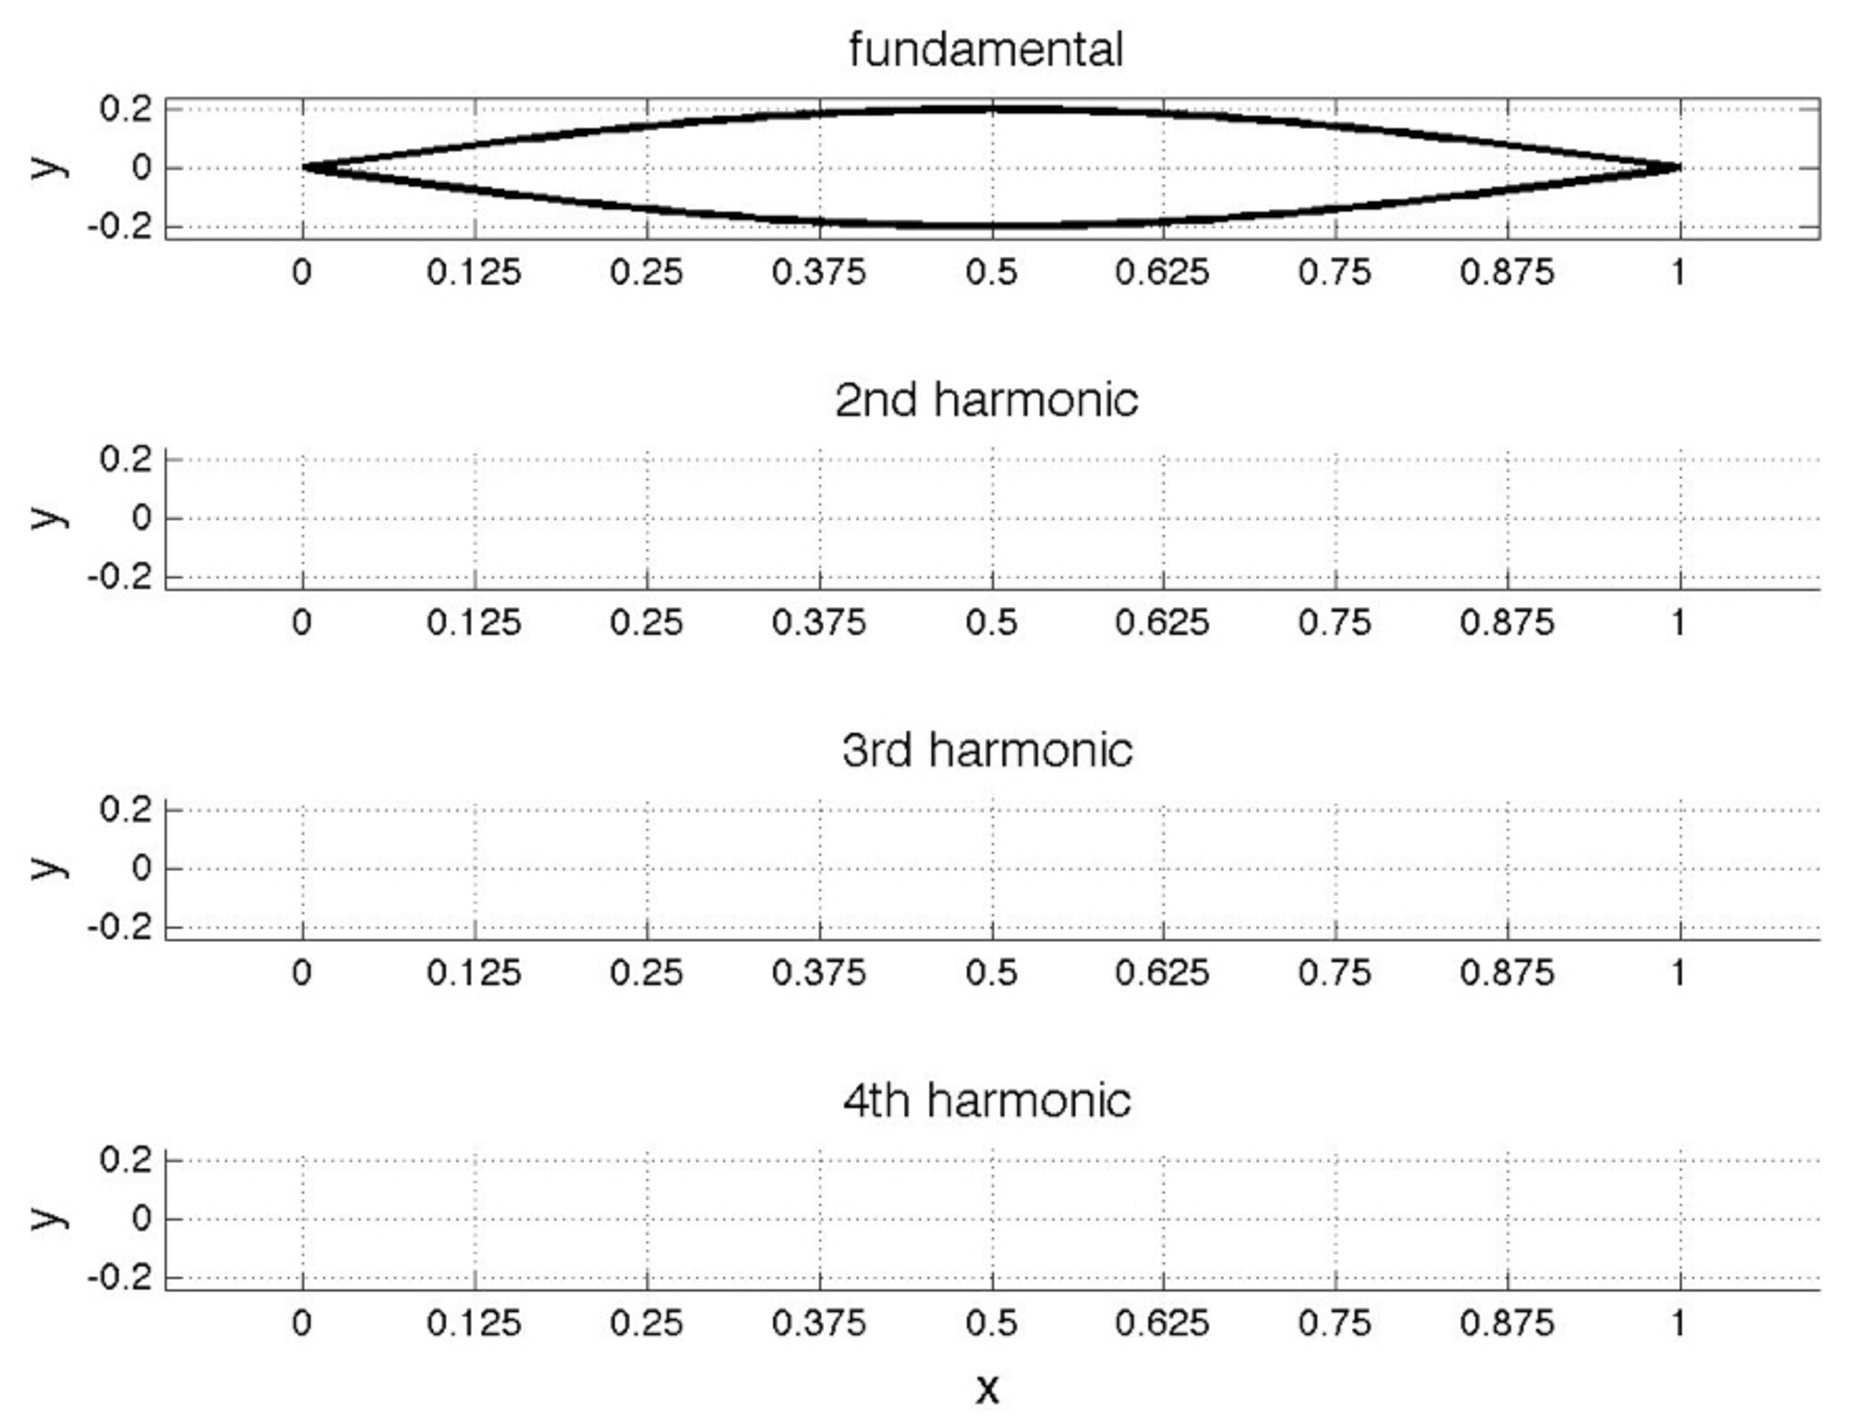
\includegraphics[width=5.5in]{standingwaves}
  %\caption{Figure caption}
  \end{center}
\end{figure}
%
\FloatBarrier

\i Standing waves are set up in the guitar string
from the Problem 4.
Calculate the value of the fundamental frequency
and the 2nd and 3rd harmonics.

\een

